\chapter{Background and Preliminary Material}

\section{About NNs}
Neural Networks can be thought of as universal function approximaters,
in fact, it has been shown that a feed-forward neural network can approximate any 
function arbitrarily closely (iff it has non-polynomial activation functions)
%TODO: \cite{universal approximation}
%TODO: clarify if sufficient depth or width is needed
There exist more complicated and exotic neural networks (e.g. RNNs, LSTMS, Encoder-Decoders, etc).

In general, throughout this paper we refer to the function induced by a given neural network
as $f(x)$ where $f:\R^n \to \R^k$.
A feed-forward neural network is composed of a series of layers of neurons \\

TODO: define artificial neuron
TODO: define layer,
TODO: define activation function,
TODO: quick clarification on what is training and how neural networks are trained \\

\section{About NN Verification}
Formally verifying the behavior of a neural network involves
proving that a 

There are several frameworks for defining neural network behavior verification.
One approach borrows from computer science and logic to define input output relations
%TODO: \cite{under-grad-paper}
The framework that we will focus on is outlined by
Bastani et al. and involves several key ideas.
%TODO: \cite{Measuring NN Robustness with Constraints}
Given a test point $x^* \in X$, with $f(x_*) = \l_*$,
then an
{\bf adversarial example}
is an input
$x_* + r \in X$ where $f(x_* + r) \neq \l_*$,
where $r$ (the adversarial perturbation) is small.

\subsection{Measures of Robustness}

For a classifier $f$ and reference input $x_*$, we say that $f$ is
{\bf $\epsilon$-robust at $x_*$}
if every $x$ within $\epsilon$ distance of $x_*$ is classified the same.
That is if $\norm{x - x_*} \leq \epsilon$ implies $f(x) = f(x_*)$,
then $f$ is $\epsilon$-robust at $x_*$
Typically, the infinity norm is used (TODO: citation and explanation).
Now we say that the
{\bf point-wise robustness of $f$ at $x_*$}
(denoted $\rho(f, x_*)$),
is the smallest $\epsilon$ for which $f$ fails to be $\epsilon$-robust at $x_*$.
\begin{equation}{}
  \rho(f, x_*)
  \medspace
  \defeq
  \medspace
  \inf
  \left\{
    \epsilon > 0 \st f
    \text{ is not }
    \epsilon\text{-robust at } x_*
  \right\}
\end{equation}

Building on this idea, we define the
{\bf adversarial frequency} of $f$
as
\begin{equation}{}
  \phi(f, \epsilon)
  \medspace
  \defeq
  \medspace
  \Pr_{x_* \sim \D}
  \left[
    \rho(f, x_*) \leq \epsilon
  \right]
\end{equation}
The distribution $\D$ from which $x_*$ is drawn
could be uniform over $X$ in the simplest case or
could reflect a prior distribution inferred from the sample data.
We can think of the adversarial frequency as
the proportion of points in the domain of $f$ that fail to be
$\epsilon$ robust.

We can further build on the central idea of point-wise robustness
to define the
{\bf adversarial severity} when $f$ is not $\epsilon$-robust at $x_*$, by
\begin{equation}{}
  \mu(f,\epsilon)
  \medspace
  \defeq
  \medspace
  \EX_{x_* \sim \D}
  \left[
    \rho(f, x_*)
    \medspace
    \st
    \medspace
    \rho(f, x_*) \leq \epsilon
  \right]
\end{equation}
TODO: give interpretation

TODO: cite Bastani
TODO: show some examples
TODO: describe computation



%\begin{figure}
%\caption{Example of a basic figure title}
%%Use the scale parameter to size the image
%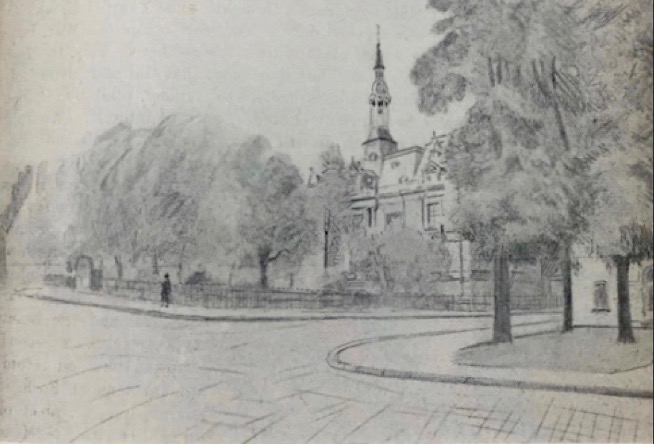
\includegraphics[width=1\textwidth]{Picture1}

%% here is an alternate way to scale images based on specific sizes
%%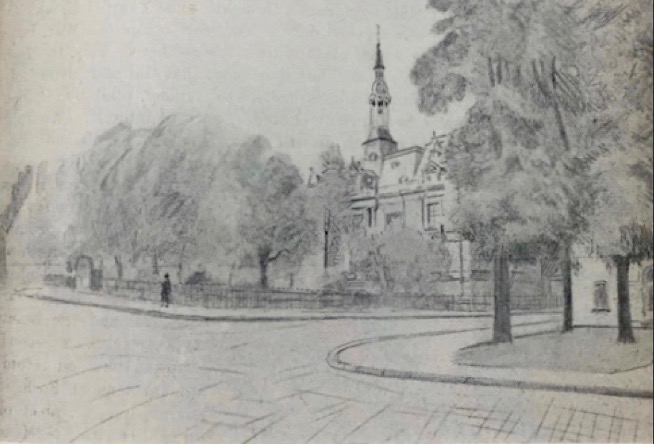
\includegraphics[width=5cm, height=4cm]{Picture1}
 %\emph{This is an example of an image caption or description}
%\end{figure}

% To remove the numeric value of the subheading below, insert an asterisk after \section ()

\section{Chapter 1 Heading 3 (subheading)}

Cras faucibus condimentum odio. Sed ac ligula. Aliquam at eros. Etiam at ligula et tellus ullamcorper ultrices. In fermentum, lorem non cursus porttitor, diam urna accumsan lacus, sed interdum wisi nibh nec nisl. Ut tincidunt volutpat urna. Mauris eleifend nulla eget mauris. Sed cursus quam id felis. Curabitur posuere quam vel nibh. Cras dapibus dapibus nisl.\par

Vestibulum quis dolor a felis congue vehicula. Maecenas pede purus, tristique ac, tempus eget, egestas quis, mauris. Curabitur non eros. Nullam hendrerit bibendum justo. Fusce iaculis, est quis lacinia pretium, pede metus molestie lacus, at gravida wisi ante at libero. Quisque ornare placerat risus. Ut molestie magna at mi. Integer aliquet mauris et nibh. Ut mattis ligula posuere velit. Nunc sagittis.\par

\subsection{\emph{Chapter 1 Heading 4 (Sub-heading)}}

Curabitur varius fringilla nisl. Duis pretium mi euismod erat. Maecenas id augue. Nam vulputate. Duis a quam non neque lobortis malesuada. Praesent euismod. Donec nulla augue, venenatis scelerisque, dapibus a, consequat at, leo. Pellentesque libero lectus, tristique ac, consectetuer sit amet, imperdiet ut, justo. Sed aliquam odio vitae tortor. Proin hendrerit tempus arcu. In hac habitasse platea dictumst. Suspendisse potenti.\par
